%-------------------------------------STYLES----------------------------------------------------------------%

\documentclass[10pt, xcolor=dvipsnames]{beamer}

%\mode<presentation>
%{
\usetheme{Madrid}
%\setbeamercovered{transparent}
%} 
%\usefonttheme{professionalfonts}
\usecolortheme{beaver}

\usepackage{setspace}
\usepackage[english]{babel}
\usepackage[latin1]{inputenc}
\usepackage{times}
\usepackage[T1]{fontenc}
\usepackage{color}
\usepackage{graphicx}
\usepackage{amssymb}
\usepackage{amsthm}
\usepackage{bm}
\usepackage{rotating}
\usepackage{ccaption}
\usepackage{booktabs}
\usepackage{lscape}
\usepackage{colortbl}
\usepackage{arydshln}
\usepackage{tabularx}
\usepackage{appendixnumberbeamer}

%\useinnertheme{rounded}
\setbeamertemplate{items}[balls]
%\usepackage[notocbib]{apacite}                % This is bibliography package.
%\renewcommand{\bibliographytypesize}{\tiny}
\setbeamertemplate{navigation symbols}{}
\usepackage{graphics}
\usepackage{epstopdf}
\DeclareGraphicsRule{.tif}{png}{.png}{`convert #1 `dirname #1`/`basename #1 .tif`.png}
%\usepackage{fleqn}
%\setlength{\mathindent}{1cm}
%\color{white}
%\hypersetup{colorlinks=true,linkcolor=Blue}
\usepackage{bbm}
\newcommand{\backupbegin}{
   \newcounter{framenumberappendix}
   \setcounter{framenumberappendix}{\value{framenumber}}
}
\newcommand{\backupend}{
   \addtocounter{framenumberappendix}{-\value{framenumber}}
   \addtocounter{framenumber}{\value{framenumberappendix}}
}

%% Change the margins
\newenvironment{changemargin}[2]{%
  \begin{list}{}{%
    \setlength{\topsep}{0pt}%
    \setlength{\leftmargin}{#1}%
    \setlength{\rightmargin}{#2}%
    \setlength{\listparindent}{\parindent}%
    \setlength{\itemindent}{\parindent}%
    \setlength{\parsep}{\parskip}%
  }%
  \item[]}{\end{list}}

\newtheorem{proposition}{Proposition}

%-------------------------------------------Title---------------------------------------------------%


\title[Land Constraints]{{How Tight are Malthusian Constraints?}}

\author[Johnson \& Vollrath]{T. Ryan Johnson \inst{1} \and Dietrich Vollrath \inst{2}}
\institute[UH]{\inst{1} University of Houston \and %
                      \inst{2} University of Houston}

\date[June 2017]{}

%-------------------------------------------Slides---------------------------------------------------%

\begin{document}
\maketitle

\section{Introduction}

\begin{frame}{Translation}\label{define}

What is the elasticity (i.e. how tight) of agricultural output with respect to land (i.e. the Malthusian constraint)? 

What we do: 
\begin{itemize}
  \item Estimate the elasticity using district-level variation in rural density
  \item Estimate separately for different climate zones, agric. type, etc..
  \item Show elasticity is 2x higher for temperate zone vs. tropics
  \item Show differences are robust w.r.t. data sources, measurement error
\end{itemize}


\end{frame}


\begin{frame}{Why do you care?}
The elasticity determines the degree of decreasing returns to scale for labor/capital in agriculture. 

\begin{itemize}
  \item \textbf{Theory}: The higher the elasticity, the more sensitive are $y$ and $L_A/L$ to shocks in population/productivity.
  \item \textbf{Evidence}: Using epidemiological transition after WWII a la Acemoglu and Johnson (2007), countries with high elasticities had more severe negative effect of rising life expectancy
  \item \textbf{Speculation}: Plays a part in explaining why temperate areas in Europe were able to accelerate development relative to Asia? 
\end{itemize}

\end{frame}

\section{Model}

\begin{frame}{Density and Productivity}
Province $I$ contains a set of districts, each denoted by $i$, with aggregate agricultural production
\begin{equation}
Y_{i} = A_{i} X_{i}^{\beta} \left(K_{Ai}^{\alpha}L_{Ai}^{1-\alpha}\right)^{1-\beta} \label{EQ_production}
\end{equation}
\begin{itemize}
  \item $A_i$ is productivity, $X_i$ is land
  \item $K_{Ai}$ is all other inputs (e.g. capital)
  \item $L_{Ai}$ is agricultural labor in district $i$ (not a single sector)
  \item Assume $\beta$ and $\alpha$ are identical \textit{within} province (but not nec. \textit{across} provinces)
\end{itemize}
\end{frame}

\begin{frame}{Agricultural Labor Allocation}
Assume that labor and capital are mobile across districts \textit{within} province (but not nec. \textit{across} provinces), and you can solve for
\begin{equation}
\ln L_{Ai}/X_i = \frac{1}{\beta} \ln A_{i} + \ln \frac{L_A}{\sum_{j\in I} A_{j}^{1/\beta}X_{j}}, \label{EQ_est}
\end{equation}
where second term is \textit{province-specific}. 

\begin{itemize}
  \item $\beta$ can be estimated from elasticity of $L_{Ai}/X_i$ w.r.t. $A_i$. 
  \item $\beta$ large (tight), $1/\beta$ small, ag. workers spread evenly w/in province
  \item $\beta$ small (loose), $1/\beta$ large, ag. workers concentrated on high $A_i$
  \item Ag labor relative to total labor ($L_A/L$) does not enter
  \item Expression is not unique to heaviliy agricultural provinces (or eras)
\end{itemize}

\hfill \hyperlink{extend}{\beamerbutton{More}}
\end{frame}

\section{Regression Setup}

\begin{frame}{Using as a Specification}
Re-arranging the prior expression and adding some notation:
\begin{equation}
  \ln A_{isc} = \alpha + \beta \ln L_{Aisc}/X_{isc} + \gamma_{sc} + \delta' \mathbf{Z}_{isc} + \epsilon_{isc}. \label{EQ_regress}
\end{equation}

\begin{itemize}
  \item District $i$, region/state/province $s$, country $c$
  \item $\gamma_{sc}$, province/country FE, pick up province-specific term
  \item $\mathbf{Z}_{isc}$ are additional controls
  \item $\epsilon_{isc}$ is error term
\end{itemize}
\end{frame}

\begin{frame}{Using as a Specification}
We moved productivity, $A_{isc}$ and agric. density $L_{Aisc}/X_{isc}$ to opposite sides:
\begin{equation}
  \ln A_{isc} = \alpha + \beta \ln L_{Aisc}/X_{isc} + \gamma_{sc} + \delta' \mathbf{Z}_{isc} + \epsilon_{isc}. \label{EQ_regress}
\end{equation}

\begin{itemize}
  \item Estimating $1/\beta$ $\Rightarrow$ very sensitive to small differences in $\beta$
\end{itemize}
\end{frame}

\begin{frame}{Agricultural Density Data}
$L_{Aisc}$ comes from HYDE 3.1 database (Goldewijk et al, 2011)
\begin{itemize}
  \item Population counts for 5 degree grid-cells built from administrative data
  \item We aggregate data back to administrative level (e.g. districts)
  \item Rural population data (not agricultural)
  \item Main samples based on year 2000
\end{itemize}
$X_{isc}$ calculated as area of a given district
\begin{itemize}
  \item Measure of possible agricultural land
\end{itemize}
$L_{Aisc}/X_{isc}$ data 
\begin{itemize}
  \item Trim above 99th and below 1st percentiles
  \item Drop if fewer than 100 total rural residents
  \item 35,451 total districts from around world
\end{itemize}
\end{frame}

\begin{frame}{Agricultural Density Data}
\begin{center}
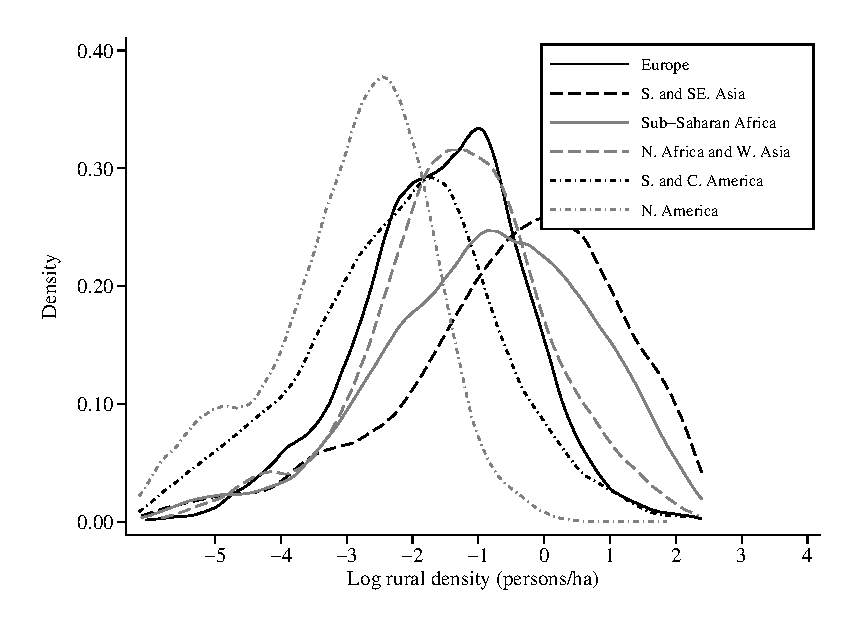
\includegraphics[width=.8\textwidth]{fig_dens_rurd.eps}
\end{center}
\end{frame}

%\begin{frame}{Agricultural Density Data}
%\begin{center}
%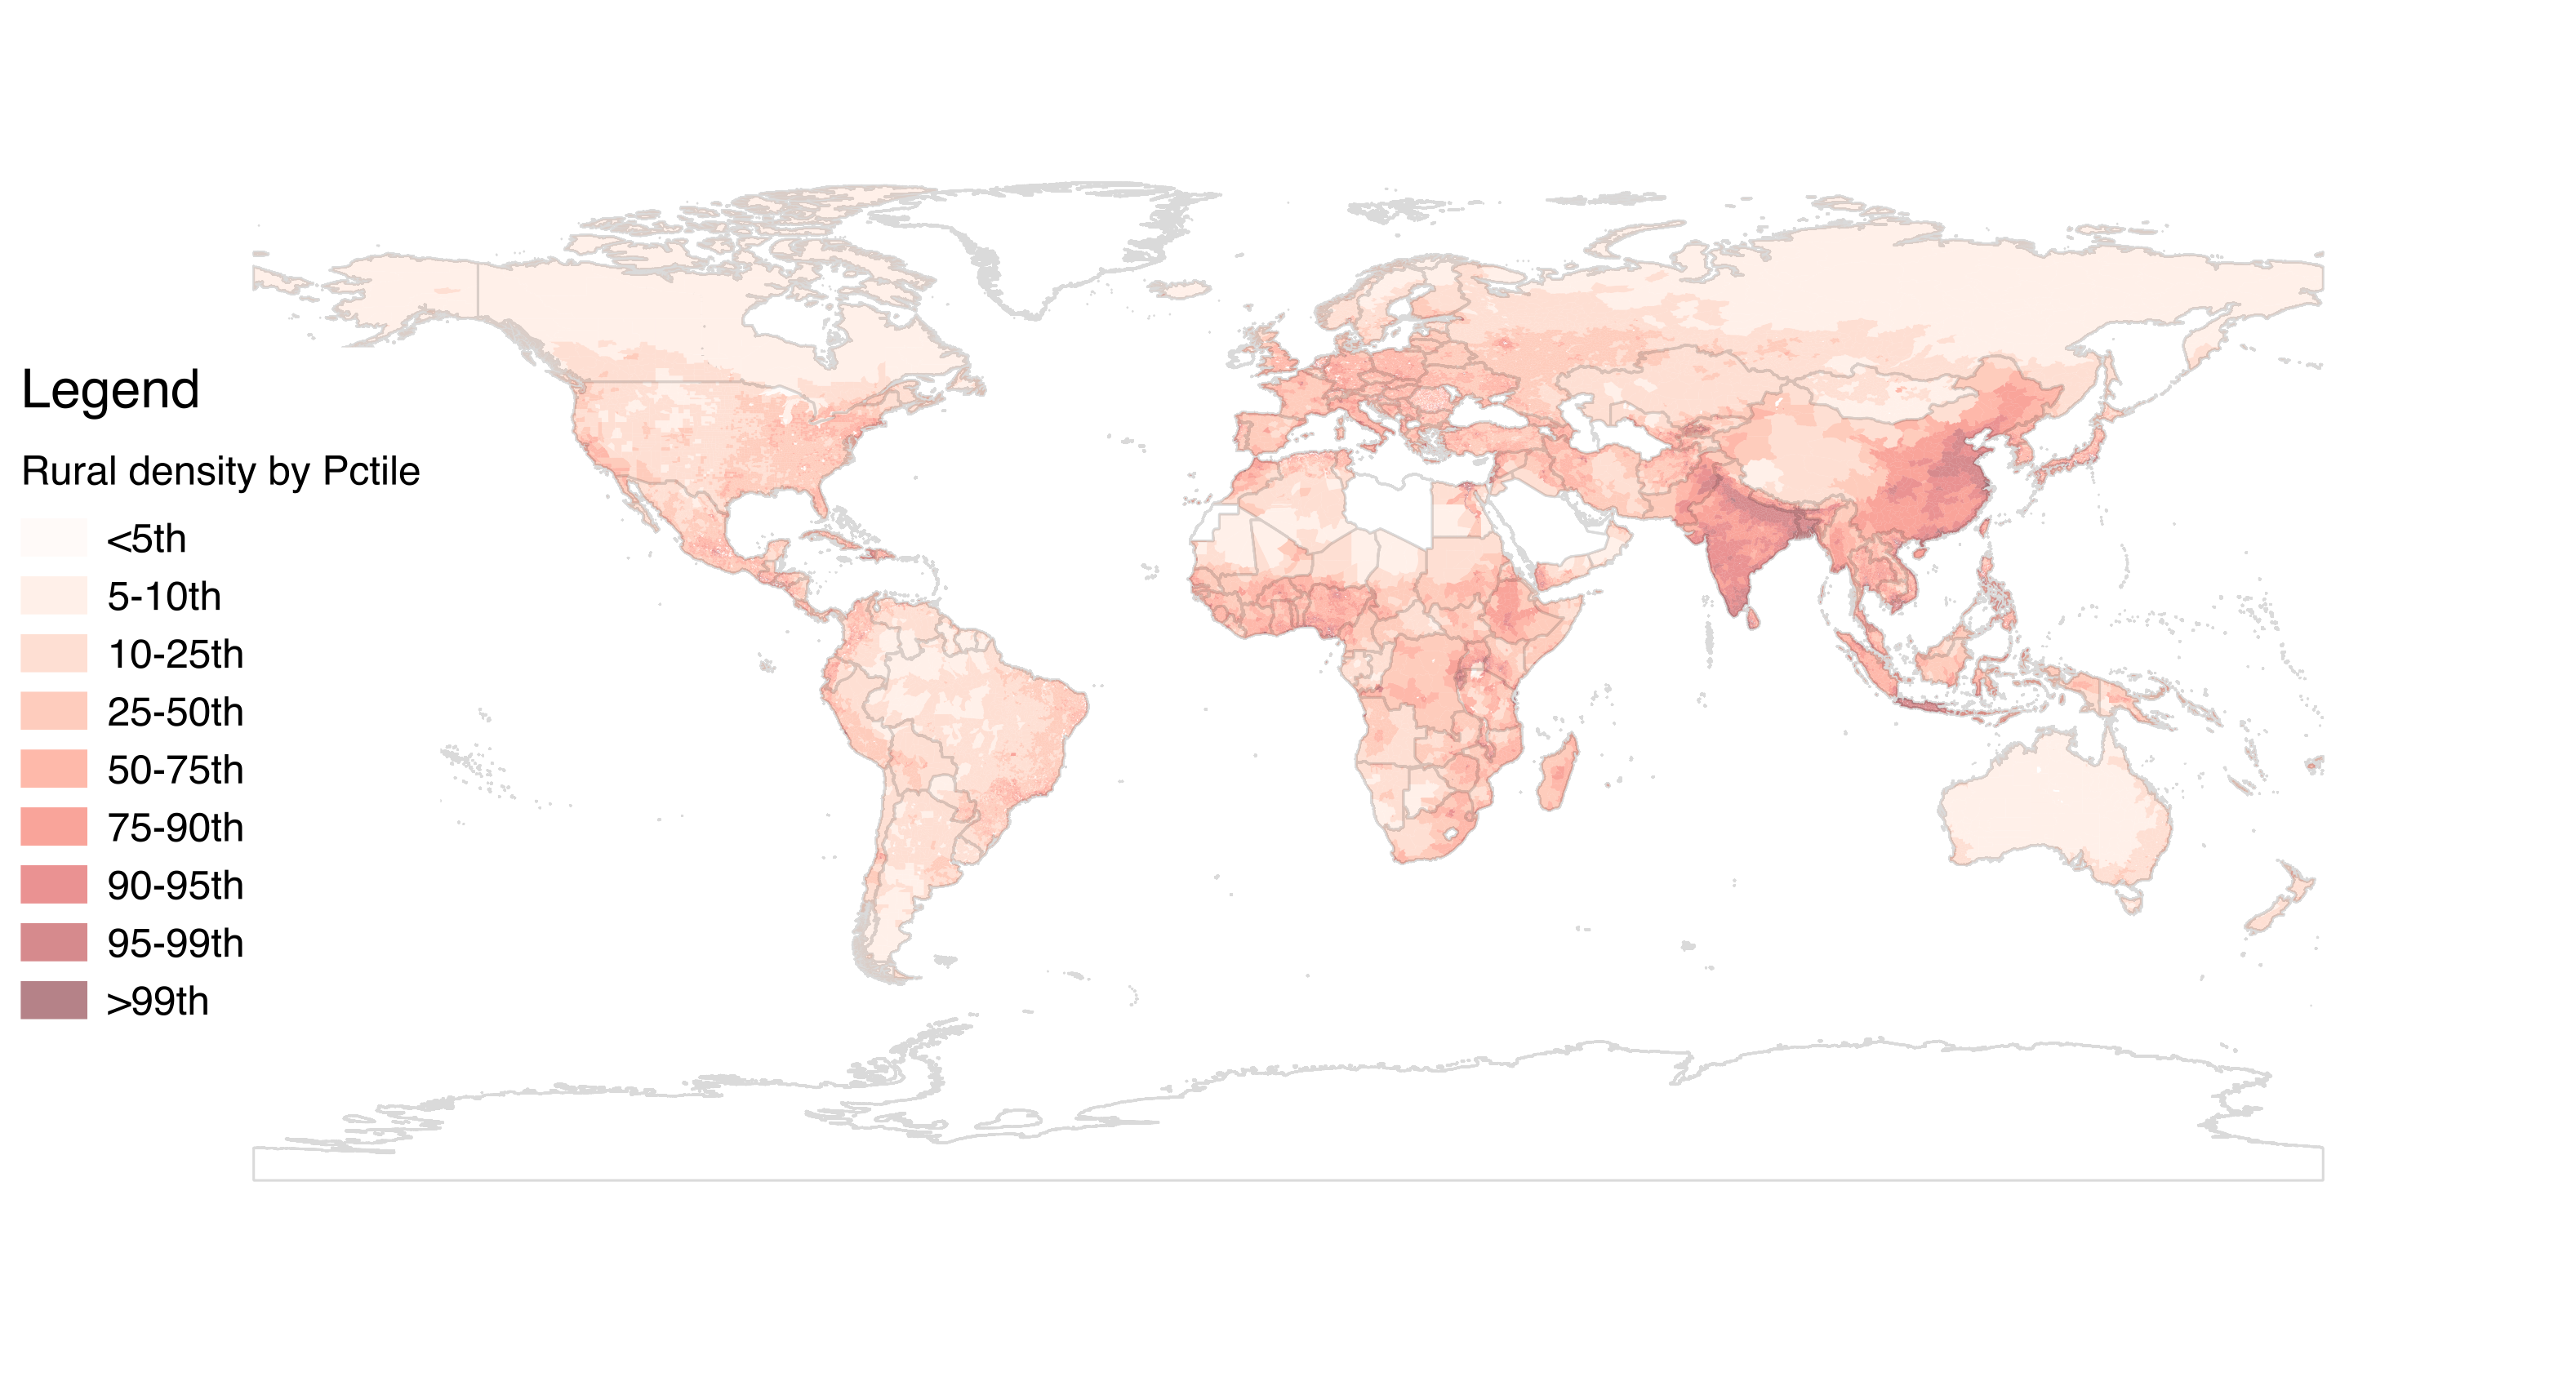
\includegraphics[scale=.5]{fig_rurd_map.png}
%\end{center}
%\end{frame}

\begin{frame}{Agricultural Productivity Data}\label{data}
$A_{isc}$ is built from Galor and {\"O}zak (2016) caloric suitability index
\begin{itemize}
  \item Data from GAEZ on agro-climatic possible yield (in raw tons) for each crop
  \item Combine with nutritional information by crop (total calories per raw ton)
  \item For each grid cell, determine max calories across all crops
  \item Sum max calories across grid cells in district, divide by total area
  \item Holds technology assumptions constant
  \item Trim above 99th and below 1st percentile
\end{itemize}
\hfill \hyperlink{stats}{\beamerbutton{Summary}}

\hfill \hyperlink{crops}{\beamerbutton{Crops}}
\end{frame}

\begin{frame}{Agricultural Productivity Data}
\begin{center}
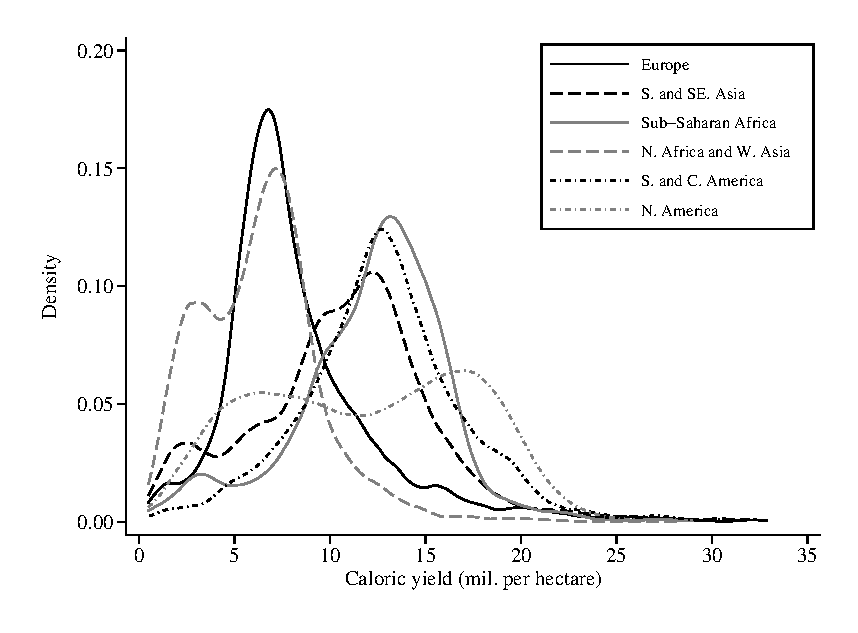
\includegraphics[width=.8\textwidth]{fig_dens_csi.eps}
\end{center}
\end{frame}

%\begin{frame}{Agricultural Productivity Data}
%Grid cells take values of their district. Shown by percentiles.
%\vspace{-.5in}
%\begin{center}
%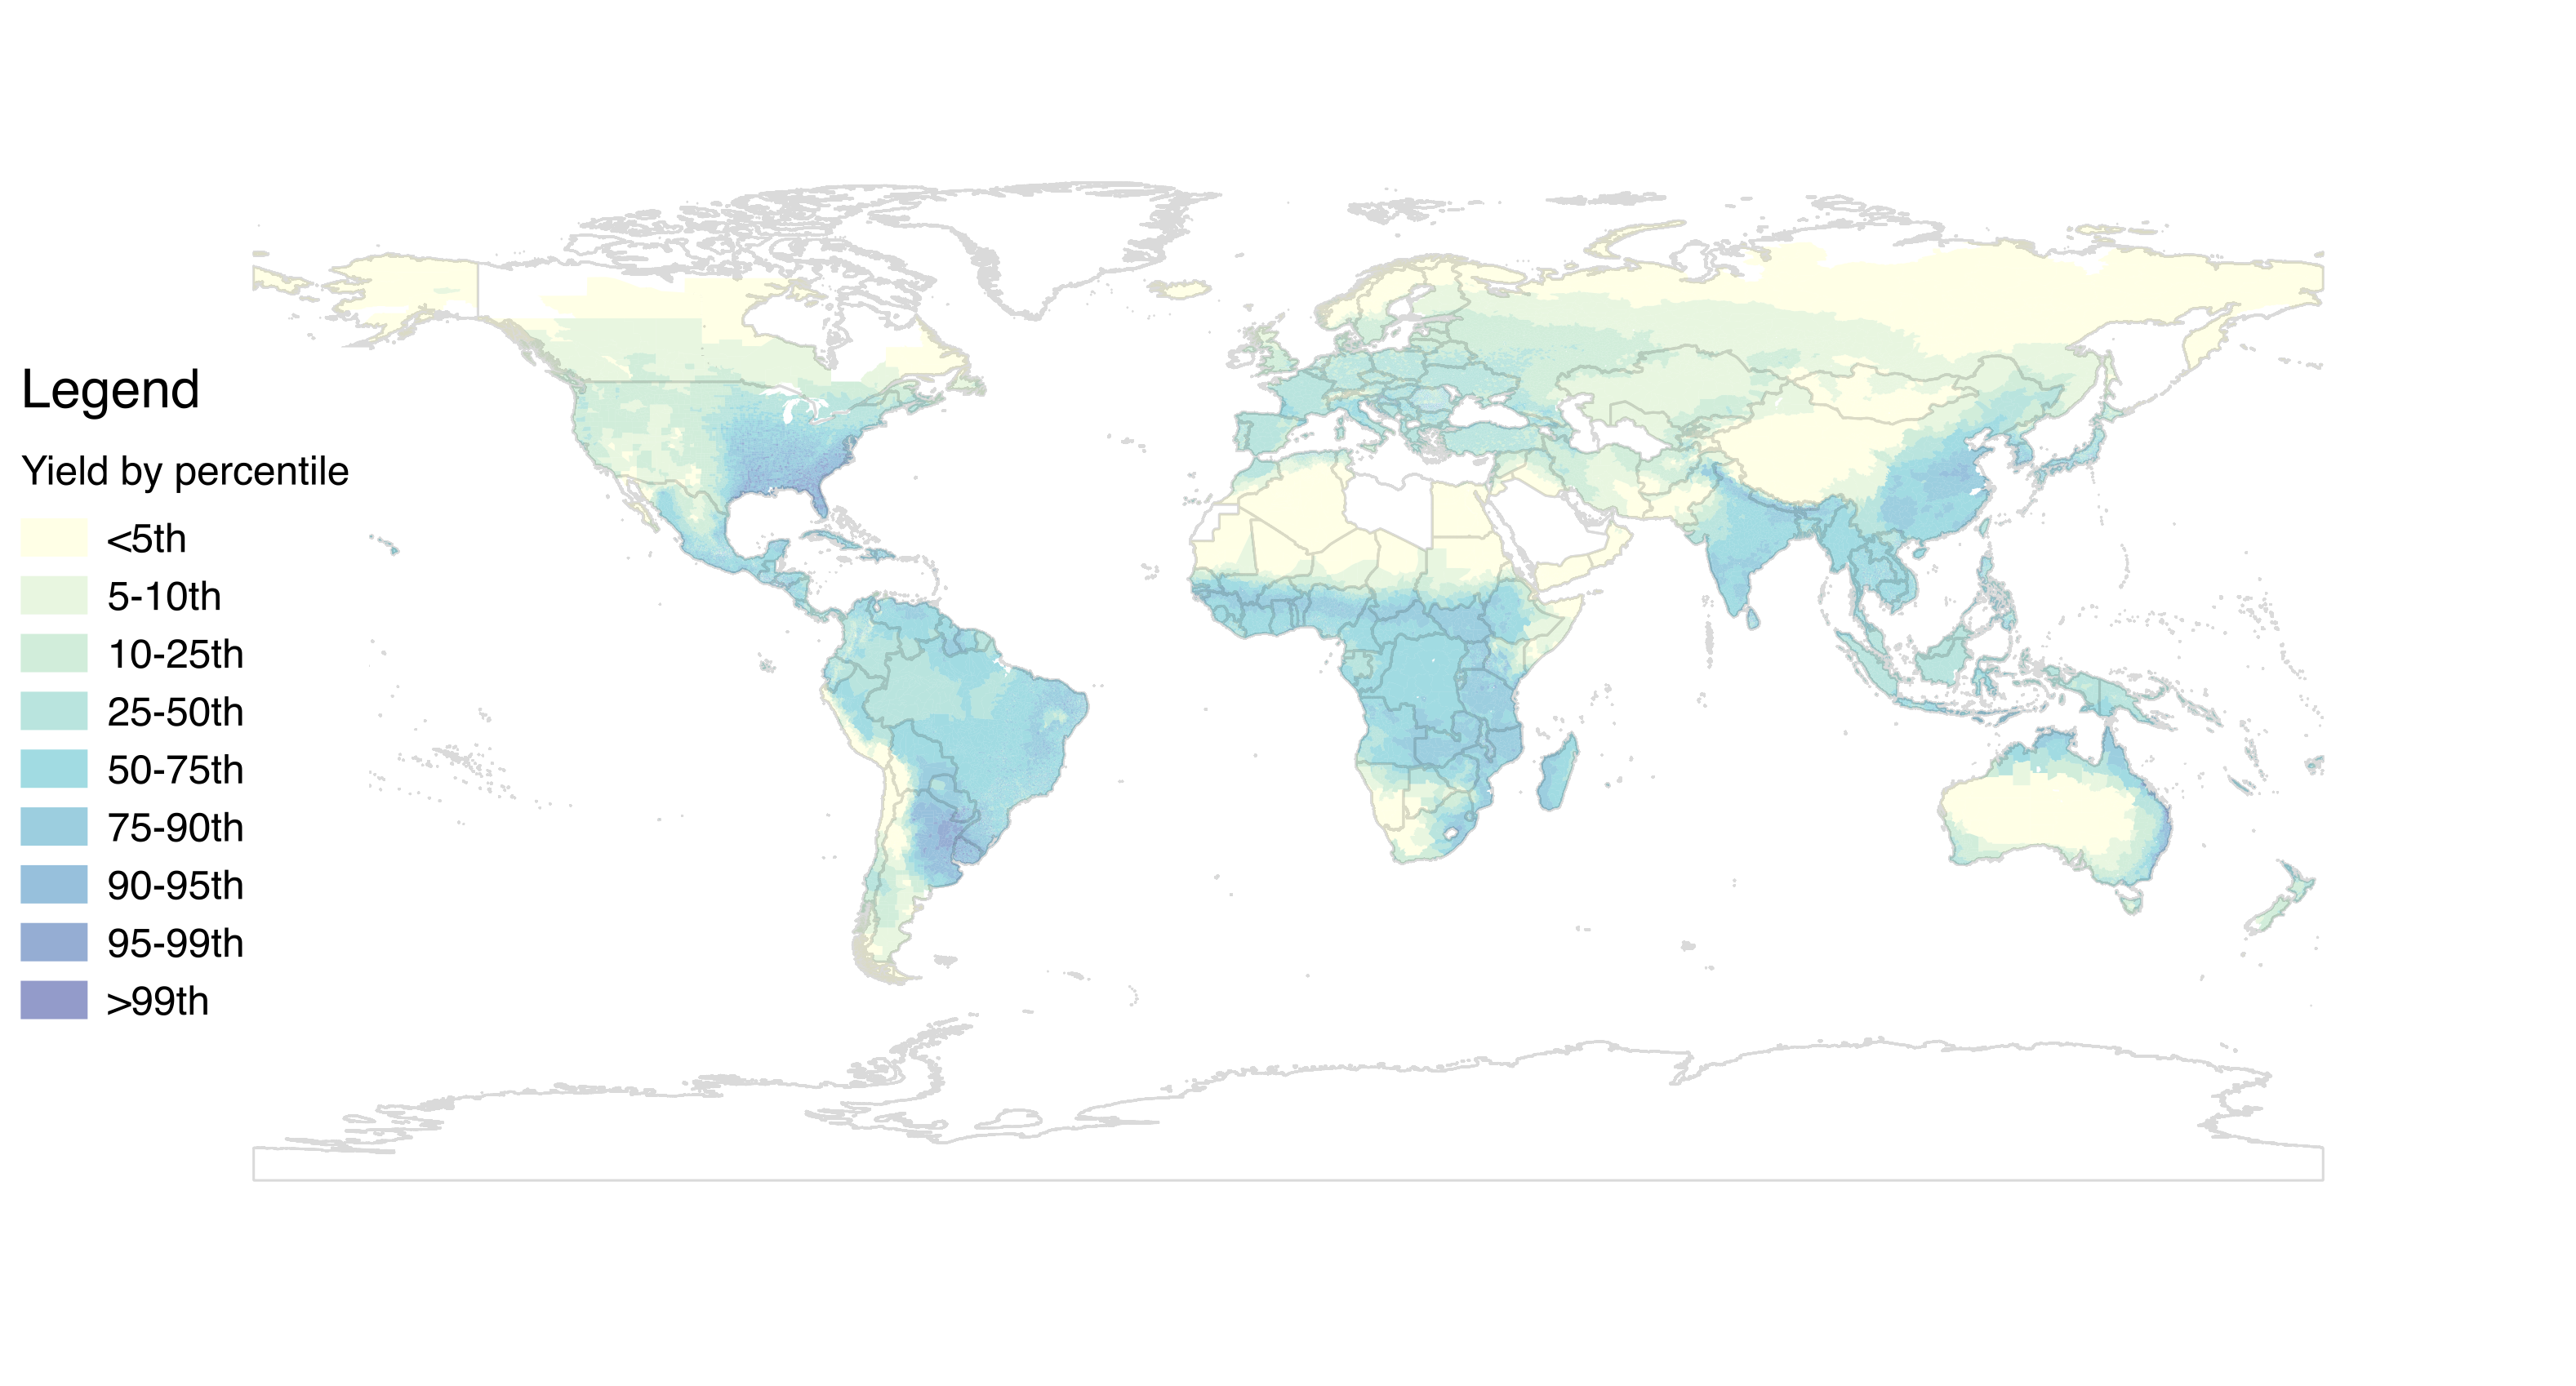
\includegraphics[scale=.5]{fig_csi_yield_map.png}
%\end{center}
%\end{frame}

\begin{frame}{Control Variables}
Henderson et al (2016) on spatial distribution of economic activity
\begin{itemize}
  \item Urban activity correlated with (caused by?) high agricultural productivity (in some places)
  \item Low rural density because of urban activity
  \item $Corr(\epsilon_{isc},\ln L_{isc}/X_{isc})<0$
\end{itemize}

Include two controls at the district level in $\mathbf{Z}_{isc}$ for urban/economic activity:
\begin{itemize}
  \item Night lights density: follows Henderson et al (2016) using Global Radiance Calibrated data
  \item Urban percent of population: from HYDE
\end{itemize}

\end{frame}

\section{Results}

%\begin{frame}{Raw Correlation for Temperate/Tropical}
%\begin{center}
%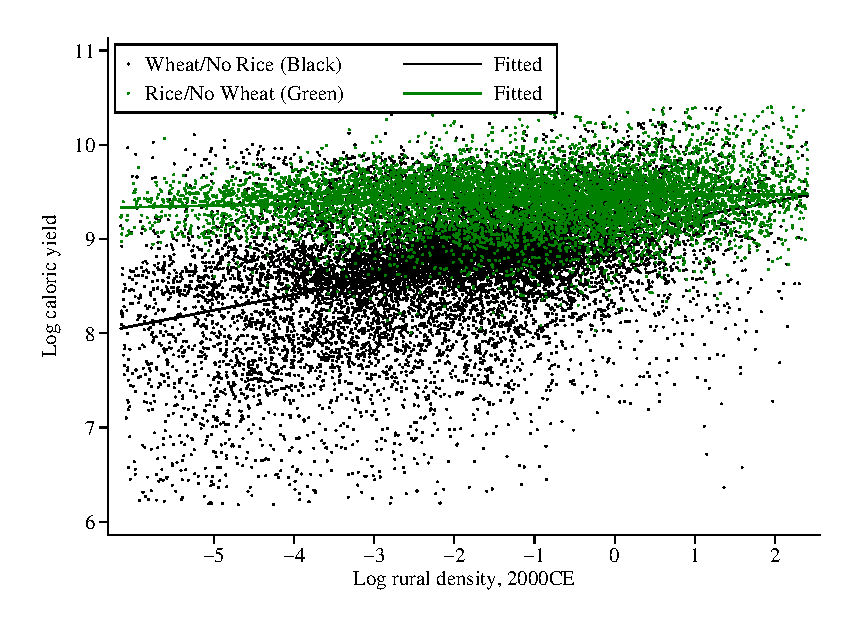
\includegraphics[width=0.8\textwidth]{fig_beta_crop.eps}
%\end{center}
%\end{frame}

\begin{frame}{``Temperate'' versus ``Tropical''}
Define the following:
\begin{itemize}
  \item \textbf{Temperate}: suitable for barley, buckwheat, rye, oats, white potatoes, and/or wheat but zero suitability for Tropical crops
  \item \textbf{Tropical}: suitable for cassava, cowpeas, pearl millet, sweet potatoes, paddy rice, and/or yams but zero suitability for Temperate crops
\end{itemize}
Measure suitability several ways
\begin{itemize}
  \item GAEZ suitability indices (0 to 100), OR
  \item Source of maximum calories in our $A_{isc}$ measure, OR
  \item Actual harvested area
\end{itemize}

\end{frame}

\begin{frame}{Results by Temperate/Tropical}\label{crop}
\begin{center}
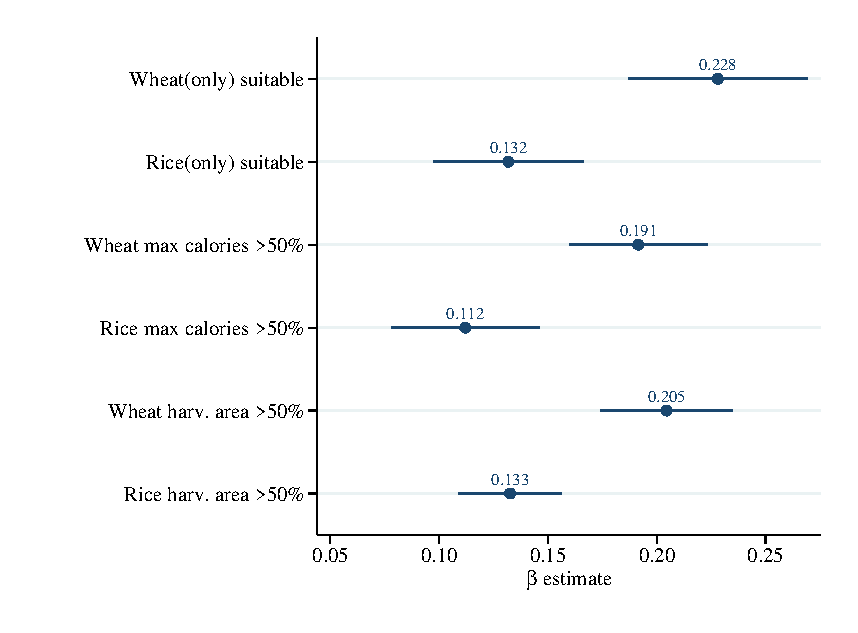
\includegraphics[width=.8\textwidth]{fig_coef_crop_base.eps}
\end{center}
\hfill \hyperlink{cropreg}{\beamerbutton{Table}}
\end{frame}

\begin{frame}{Results by Temperate/Tropical}
\begin{center}
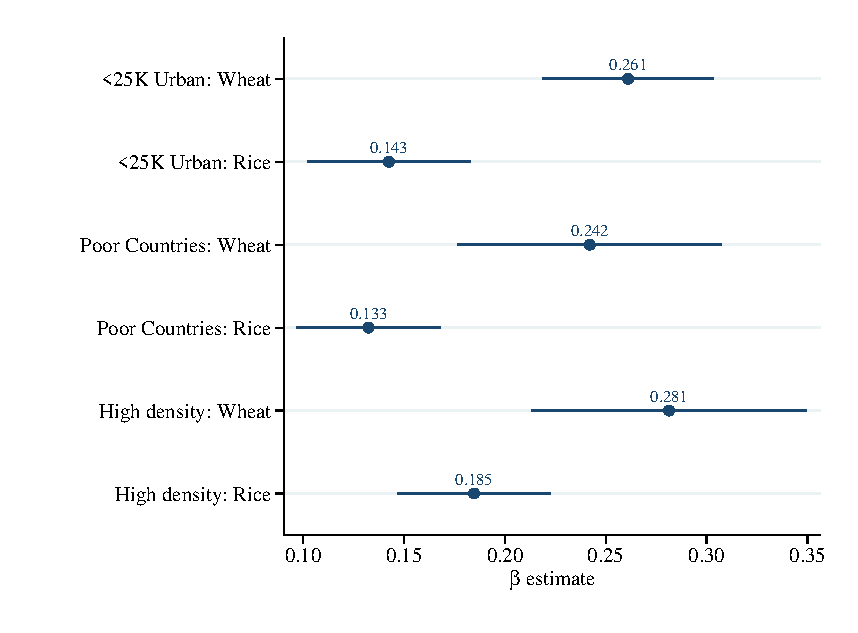
\includegraphics[width=.8\textwidth]{fig_coef_crop_sub_base.eps}
\end{center}
\end{frame}

\begin{frame}{Results by Climate Zone}
Look at specific climate factors, rather than agricultural crops grown
\begin{itemize}
  \item Create samples based on K{\"o}ppen-Geiger zones
  \item Three layers: Climate, Precipitation, Temperature
  \item Each layer has multiple types (e.g. Climate is Equatorial, Arid, ...)
  \item Create samples where districts have >50\% of land in a given type
  \item $\Rightarrow$ heterogeneity within countries in $\beta$  
\end{itemize}
\end{frame}

\begin{frame}{Results by Climate Zone}\label{climate}
\begin{center}
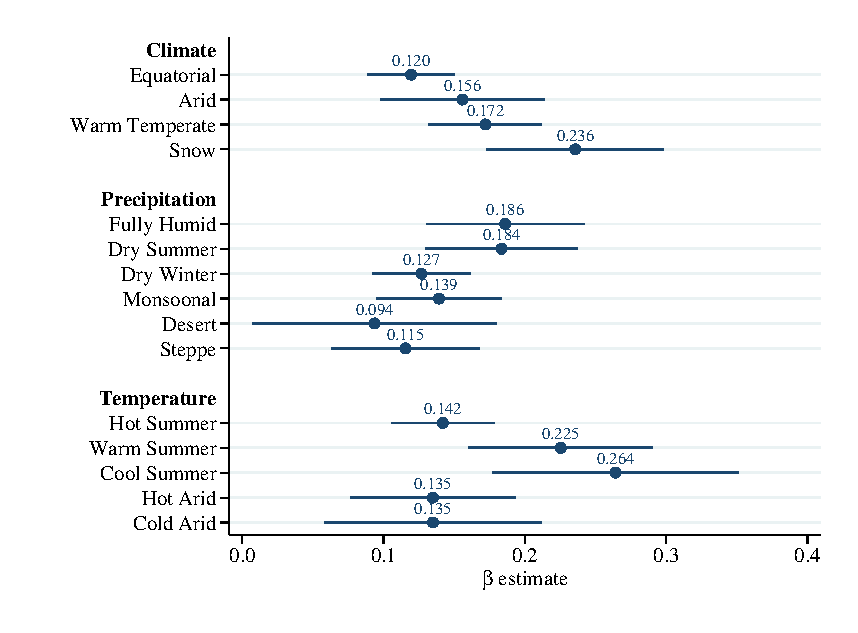
\includegraphics[width=.8\textwidth]{fig_coef_kg_base.eps}
\end{center}
\hfill \hyperlink{climatereg}{\beamerbutton{Table}}
\end{frame}

\begin{frame}{Results by Sub-Region}\label{subregion}
\begin{center}
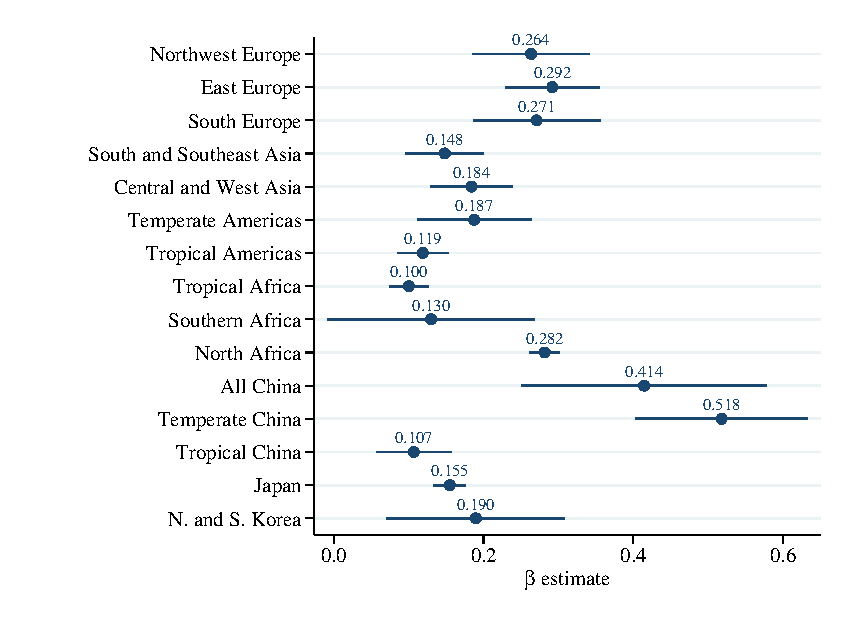
\includegraphics[width=.8\textwidth]{fig_coef_subregion_base.eps}
\end{center}
\hfill \hyperlink{subregiontab}{\beamerbutton{Table}}
\end{frame}

%\begin{frame}{Explanations?}
%Evidence suggests:
%\begin{itemize}
%  \item Tight constraints: wheat family, temperate/snow, warm/cool summers
%  \item Loose constraints: rice family, equatorial/arid, hot summer/arid
%\end{itemize}
%
%\vspace{.2cm} Why looser constraints some areas?
%\begin{itemize}
%  \item Positive(?): Multiple cropping, longer growing periods, more sun, more rain during growing periods $\Rightarrow$ land area isn't binding?
%  \item Negative(?): Soil leaching, lack of frost $\Rightarrow$ land is less useful?
%\end{itemize}

%\vspace{.2cm} Working on new project that uses actual crop yields to back out elasticities \textit{by crop} within a given grid cell, with constant climate conditions
%\end{frame}

\begin{frame}{Robustness and questions}\label{robustness}
\begin{itemize}
  \item Use province level data (with country FE) \hyperlink{regprov}{\beamerbutton{Results}}
  \item Use rural density from 1900 from HYDE \hyperlink{reg1900}{\beamerbutton{Results}}
  \item Use IPUMS for agricultural population \hyperlink{ipums}{\beamerbutton{Results}}
  \item Use GRUMP for population data \hyperlink{grump}{\beamerbutton{Results}}
  \item Estimate $\beta$ for individual provinces \hyperlink{prov}{\beamerbutton{Results}}
  \item Use cultivated area of land \hyperlink{cultreg}{\beamerbutton{Results}}
  \item Maize and soy \hyperlink{othercrop}{\beamerbutton{Results}}
  \item Exclude districts with few harvest Ha \hyperlink{harvarea}{\beamerbutton{Results}}
  \item Workers not mobile between districts? \hyperlink{nonmobile}{\beamerbutton{Slides}}
  \item Districts autarkic? \hyperlink{autarky}{\beamerbutton{Slides}}  
  \item Elasticity of substitution? \hyperlink{eos}{\beamerbutton{Slides}}
  \item Measurement error? \hyperlink{measure}{\beamerbutton{Slides}}
  \item Factor shares? \hyperlink{shares}{\beamerbutton{Slides}}
\end{itemize}
\end{frame}

\section{Implications}

\begin{frame}{Back to the model}\label{extend}
Summarizing:
\begin{itemize}
  \item Preferences for ag/non-ag goods (Boppart, 2014). $\epsilon > \gamma$ are parameters ensuring income elasticity for ag is less than one, and ag/non-ag are substitutes. This ensures that productivity improvements in any sector drive down ag labor share.
  \item Non-ag sector is CD with capital and labor only. Ag sector is as described.
  \item Static. Not thinking about transition paths, just steady states.
  \item Focus on ag labor share ($L_A/L$) and real income per capita, $y$
\end{itemize}

\end{frame}

\begin{frame}{Elasticities}
The elasticities of the agricultural labor share ($L_A/L$) and real income ($y$) with respect to various shocks,
\begin{enumerate}
  \item[(a)] Agricultural productivity ($A_A$): 
\begin{equation}
  \frac{\partial \ln L_A/L}{\partial \ln A_A} = - \frac{\gamma}{1-\beta\gamma} \quad \quad \frac{\partial \ln y}{\partial \ln A_A} = \frac{1}{1-\beta\gamma}
\end{equation}
  \item[(b)] Non-agricultural productivity ($A_N$): 
\begin{equation}
  \frac{\partial \ln L_A/L}{\partial \ln A_N} = - \frac{\epsilon-\gamma}{1-\beta\gamma} \quad \quad \frac{\partial \ln y}{\partial \ln A_N} = \frac{\beta(\epsilon-\gamma)}{1-\beta\gamma}
\end{equation}
  \item[(c)] Population ($L$): 
\begin{equation}
  \frac{\partial \ln L_A/L}{\partial \ln L} = \frac{\beta\gamma}{1-\beta\gamma} \quad \quad \frac{\partial \ln y}{\partial \ln L} = - \frac{\beta}{1-\beta\gamma}
\end{equation}
\end{enumerate}
are all increasing in absolute value with $\beta$.
\end{frame}

\begin{frame}{Speculative implications:}
Three settings where the Malthusian constraint might matter
\begin{itemize}
  \item \textbf{Effect of Black Death:} Large effects on European development (Voigtl{\"a}nder and Voth, 2013a,b) due to tight constraint? Similar epidemics in Asia w/o major changes due to loose constraint?
  \item \textbf{Involution:} Higher densities and output, but not living standards, in response to productivity (Geertz, 1963; Huang, 1990) due to loose constraint?
  \item \textbf{Response to agric. technology/inputs:} Necessary increase to match rich countries in TFP/inputs is larger with loose constraint (Eberhardt and Vollrath, 2016a,b)
\end{itemize}
\end{frame}

\begin{frame}{Empirical implications:}
Acemoglu and Johnson (2007) analysis of epidemiological transition:
\begin{itemize}
  \item WHO (and other) interventions lower mortality rates from many tropical diseases
  \item They find higher resulting population was negative for income per capita
  \item According to our theory, the negative effect should be \textit{bigger} for places with \textit{tighter} land constraints
  \item We divide countries in AJ into ``loose'' and ``tight'' groups based on country-specific elasticities, run AJ analysis separately for those groups
\end{itemize}

Run panel regressions of form
\begin{equation}
    y_{it} = \alpha + \theta x_{it} + \gamma_i + \delta_t + \epsilon_{it}
\end{equation}
for country $i$ and time (decade) $t$. $x_{it}$ is mortality rate, (log) life expect, or (log) population size. $y_{it}$ is (log) GDP per capita, (log) GDP per worker, or (log) population.

\end{frame}

\begin{frame}{Response to mortality rate changes}

{\footnotesize
\begin{tabularx}{\textwidth}{lXXXXXX}
\midrule
 & \multicolumn{6}{c}{Dependent Variable:} \\ \cmidrule(lr){2-7}
 & \multicolumn{2}{c}{Log GDP per capita} & \multicolumn{2}{c}{Log GDP per worker} & \multicolumn{2}{c}{Log population} \\ \cmidrule(lr){2-3} \cmidrule(lr){4-5} \cmidrule(lr){6-7}
 & Loose & Tight & Loose & Tight & Loose & Tight \\
 & (1) & (2) & (3) & (4) & (5) & (6) \\
\midrule
 & \multicolumn{6}{c}{Panel A:} \\ \cmidrule(lr){2-7}
Mortality rate      &       0.333&       0.723&       0.284&       0.776&      -0.361&      -0.597\\
                    &     (0.271)&     (0.136)&     (0.262)&     (0.145)&     (0.186)&     (0.152)\\
\midrule
p-value $\theta=0$  &       0.220&       0.000&       0.281&       0.000&       0.054&       0.000\\
p-value $\theta=\theta^{Loose}$&           .&       0.199&           .&       0.102&           .&       0.327\\
Countries           &          16&          16&          16&          16&          16&          16\\
Observations        &         128&         128&         128&         128&         128&         128\\

\midrule

\end{tabularx}
}
\end{frame}

\begin{frame}{Response to life expectancy changes}

{\footnotesize
\begin{tabularx}{\textwidth}{lXXXXXX}
\midrule
 & \multicolumn{6}{c}{Dependent Variable:} \\ \cmidrule(lr){2-7}
 & \multicolumn{2}{c}{Log GDP per capita} & \multicolumn{2}{c}{Log GDP per worker} & \multicolumn{2}{c}{Log population} \\ \cmidrule(lr){2-3} \cmidrule(lr){4-5} \cmidrule(lr){6-7}
 & Loose & Tight & Loose & Tight & Loose & Tight \\
 & (1) & (2) & (3) & (4) & (5) & (6) \\
\midrule
 & \multicolumn{6}{c}{Panel B:} \\ \cmidrule(lr){2-7}
Log life expectancy &       0.309&      -2.007&       0.214&      -1.928&       1.910&       1.564\\
                    &     (0.393)&     (0.308)&     (0.387)&     (0.309)&     (0.235)&     (0.229)\\
\midrule
p-value $\theta=0$  &       0.434&       0.000&       0.582&       0.000&       0.000&       0.000\\
p-value $\theta=\theta^{Below}$&           .&       0.000&           .&       0.000&           .&       0.292\\
Countries           &          13&          14&          13&          14&          13&          14\\
Observations        &          99&         106&          99&         106&          99&         106\\

\midrule

\end{tabularx}
}
\end{frame}

\begin{frame}{Response to population change}

{\footnotesize
\begin{tabularx}{\textwidth}{lXXXXXX}
\midrule
 & \multicolumn{6}{c}{Dependent Variable:} \\ \cmidrule(lr){2-7}
 & \multicolumn{2}{c}{Log GDP per capita} & \multicolumn{2}{c}{Log GDP per worker} & \multicolumn{2}{c}{Log population} \\ \cmidrule(lr){2-3} \cmidrule(lr){4-5} \cmidrule(lr){6-7}
 & Loose & Tight & Loose & Tight & Loose & Tight \\
 & (1) & (2) & (3) & (4) & (5) & (6) \\
\midrule
 & \multicolumn{6}{c}{Panel C:} \\ \cmidrule(lr){2-7}
Log population      &      -0.380&      -0.776&      -0.383&      -0.763\\
                    &     (0.125)&     (0.067)&     (0.121)&     (0.062)\\
\midrule
p-value $\theta=0$  &       0.003&       0.000&       0.002&       0.000\\
p-value $\theta=\theta^{Below}$&           .&       0.006&           .&       0.006\\
Countries           &          16&          16&          16&          16\\
Observations        &         128&         128&         128&         128\\

\midrule

\end{tabularx}
}
\end{frame}

\section{Conclusion}

\begin{frame}{Conclusion}
\begin{itemize}
  \item Estimate Malthusian constraint - elasticity of agricultural output w.r.t. land - from variation in rural density within provinces
  \item Constraint is ``tight'' (0.20-0.30) in temperate areas (N. China, Europe, US/Canada, S. Africa)
  \item Constraint is ``loose'' (0.10-0.15) in tropical areas (S. China, SE Asia, C. Africa, S/C America)
  \item Constraint affects the sensitivity of $L_A/L$ and living standards to population and productivity
  \item Evidence from epidemiological transition is consistent with our findings and theory
\end{itemize}
\end{frame}

\section{Appendix Slides}
\appendix

\subsection{Additional information}
\begin{frame}{Interaction Regression}\label{interaction}
Combine a given sample with the reference sample (denoted by $Ref$). Run the following regression with interaction terms
\begin{eqnarray}
    \ln A_{isc} = \beta \ln L_{Aisc}/X_{isc} + (\beta^{Ref} - \beta) \ln L_{Aisc}/X_{isc} \times I(Ref) \\ \nonumber
    + \gamma_{sc} + \delta' \mathbf{Z}_{isc} + (\delta^{Ref} - \delta)'\mathbf{Z}_{isc} \times I(Ref) + \epsilon_{isc}. \label{EQ_interaction}
\end{eqnarray}
where $I(Ref)$ is an indicator for the reference region. Our hypothesis test is $H_0: \beta^{Ref} - \beta = 0$, the coefficient on the interaction term for rural density. 

\hfill \hyperlink{testing}{\beamerbutton{Return}}
\end{frame}

\begin{frame}{Summary statistics}\label{stats}
{\scriptsize
\begin{tabularx}{\textwidth}{lXXXXXXX}
\midrule
 &      &            & \multicolumn{5}{c}{Percentiles:} \\ \cmidrule{4-8}
 & Mean & SD  & 10th    & 25th    & 50th & 75th & 90th \\
\midrule
Labor/land (persons/ha) &     0.73&     1.17&     0.04&     0.12&     0.32&     0.77&     1.86\\
Caloric yield (mil cals/ha) &    10.85&     4.89&     4.98&     7.17&    10.65&    13.86&    17.03\\
Log light density &    -2.82&     2.93&    -6.14&    -3.83&    -2.51&    -0.89&     0.35\\

\midrule
\end{tabularx}
}

\hfill \hyperlink{data}{\beamerbutton{Return}}
\end{frame}

\begin{frame}{Crops used in productivity calculation}\label{crops}
alfalfa, banana, barley, buckwheat, cassava, chickpea, cowpea, drypea, flax, foxtail millet, greengram, groundnut, indica rice, maize, oat, pearl millet, phaselous bean, pigeon pea, rye, sorghum, soybean, spring wheat, sweetpotato, rape, wet/paddy rice, wheat, winter wheat, white potato, and yams

\hfill \hyperlink{data}{\beamerbutton{Return}}
\end{frame}

\subsection{Main results}


\begin{frame}{Crop Results}\label{cropreg}
{\footnotesize
\begin{tabularx}{\textwidth}{lXXXXXX}
\midrule
\multicolumn{7}{l}{Dependent Variable in all panels: Log caloric yield ($A_{isc}$)} \\ \\
\multicolumn{7}{l}{Panel A: Samples defined by crop family (wheat vs. rice):} \\ \\
 & \multicolumn{2}{c}{By suitability:} & \multicolumn{2}{c}{By max calories:} & \multicolumn{2}{c}{By harvest area:}\\ \cmidrule(lr){2-3} \cmidrule(lr){4-5} \cmidrule(lr){6-7} 
 & Wheat & Rice & Wheat  & Rice  & Wheat  & Rice \\
 & Only & Only &  $>33\%$ & $>33\%$ & $>50\%$ & $>50\%$   \\
 & (1) & (2) & (3) & (4) & (5) & (6) \\
\midrule
Log labor/land ratio ($\beta_g$)&       0.239&       0.088&       0.218&       0.093&       0.220&       0.081\\
                    &     (0.045)&     (0.020)&     (0.039)&     (0.012)&     (0.049)&     (0.016)\\
\midrule
p-value $\beta_g=0$ &       0.000&       0.000&       0.000&       0.000&       0.000&       0.000\\
p-value $\beta_g=\beta_{Temp}$&            &       0.002&            &       0.002&            &       0.007\\
Countries           &          84&          76&          91&         101&          86&          78\\
Observations        &        9404&        7229&       15260&       14794&       10221&       10013\\
R-square (ex. FE)   &        0.24&        0.20&        0.21&        0.18&        0.23&        0.18\\

\midrule
\end{tabularx}
}

\hfill \hyperlink{crop}{\beamerbutton{Return}}
\end{frame}

\begin{frame}{Crop Results}

{\footnotesize
\begin{tabularx}{\textwidth}{lXXXXXX}
\midrule
\multicolumn{7}{l}{Dependent Variable in all panels: Log caloric yield ($A_{isc}$)} \\ \\
\multicolumn{7}{l}{Panel B: Samples with other restrictions (using suitability to distinguish crop families)} \\ \\
 & \multicolumn{2}{c}{Urban Pop. $<25K$:} & \multicolumn{2}{c}{Ex. Europe/N. Amer.:} & \multicolumn{2}{c}{Rural dens. $>$ 25th P'tile:}\\ \cmidrule(lr){2-3} \cmidrule(lr){4-5} \cmidrule(lr){6-7}
  & Wheat Only& Rice Only & Wheat Only& Rice Only& Wheat Only& Rice Only\\
 & (1) & (2) & (3) & (4) & (5) & (6) \\
\midrule
Residuals           &       0.257&       0.140&       0.223&       0.131&       0.215&       0.128\\
                    &     (0.022)&     (0.021)&     (0.032)&     (0.018)&     (0.021)&     (0.020)\\
\midrule
p-value $\beta=0$   &       0.000&       0.000&       0.000&       0.000&       0.000&       0.000\\
p-value $\beta=\beta_{Temp}$&            &       0.000&            &       0.009&            &       0.003\\
Countries           &          83&          75&          24&          70&          82&          66\\
Observations        &        7648&        6662&         824&        8826&        8084&        6611\\
Adjusted R-square   &        0.29&        0.24&        0.16&        0.14&        0.24&        0.20\\

\midrule
\end{tabularx}
}
\end{frame}

\begin{frame}{Climate Results}\label{climatereg}

{\footnotesize
\begin{tabularx}{\textwidth}{lXXXXXX}
\midrule
\multicolumn{7}{l}{Dependent Variable in all panels: Log caloric yield ($A_{isc}$)} \\ \\
\multicolumn{7}{l}{Panel A: Climate Zones} \\
 & Equatorial & Arid & Temperate & Snow  &     &   \\
 & (1) & (2) & (3) & (4) &  & \\
\midrule
Log labor/land ratio ($\beta_g$)&       0.142&       0.226&       0.207&       0.140&       0.190\\
                    &     (0.021)&     (0.053)&     (0.076)&     (0.035)&     (0.046)\\
\midrule
p-value $\beta=0$   &       0.000&       0.000&       0.007&       0.000&       0.000\\
p-value $\beta=\beta_{Humid}$&            &       0.065&       0.405&       0.969&       0.254\\
Countries           &          57&          82&          18&          42&          25\\
Observations        &        8101&        9003&         340&        1230&         956\\
R-square (ex. FE)   &        0.20&        0.23&        0.20&        0.17&        0.21\\

\midrule
\end{tabularx}
}

\hfill \hyperlink{climate}{\beamerbutton{Return}}
\end{frame}

\begin{frame}{Climate Results}

{\footnotesize
\begin{tabularx}{\textwidth}{lXXXXXX}
\midrule
\multicolumn{7}{l}{Panel B: Precipitation Zones} \\
& Fully     & Dry         & Dry        &              &            & \\
& Humid & Summer & Winter & Monsoon & Desert & Steppe \\
 & (1) & (2) & (3) & (4) & (5) & (6) \\
\midrule
Log labor/land ratio ($\beta_g$)&       0.240&       0.215&       0.124&       0.125&       0.130&       0.147\\
                    &     (0.044)&     (0.063)&     (0.022)&     (0.039)&     (0.072)&     (0.029)\\
\midrule
p-value $\beta=0$   &       0.000&       0.001&       0.000&       0.001&       0.072&       0.000\\
p-value $\beta=\beta_{Humid}$&            &       0.739&       0.020&       0.043&       0.190&       0.072\\
Countries           &          78&          37&          67&          32&          20&          49\\
Observations        &       13545&        2373&        7695&        1267&         146&        1735\\
R-square (ex. FE)   &        0.17&        0.17&        0.15&        0.17&        0.17&        0.16\\

\midrule
\end{tabularx}
}

\end{frame}

\begin{frame}{Climate Results}

{\footnotesize
\begin{tabularx}{\textwidth}{lXXXXXX}
\midrule
\multicolumn{7}{l}{Panel C: Temperature Zones} \\
    & Hot        & Warm        & Cool       & Hot      & Cold     &  \\
    & Summer & Summer & Summer & Arid & Arid &   \\
 & (1) & (2) & (3) & (4) & (5) &  \\    
\midrule
Log labor/land ratio ($\beta_g$)&       0.142&       0.226&       0.207&       0.140&       0.190\\
                    &     (0.021)&     (0.053)&     (0.076)&     (0.035)&     (0.046)\\
\midrule
p-value $\beta=0$   &       0.000&       0.000&       0.007&       0.000&       0.000\\
p-value $\beta=\beta_{Humid}$&            &       0.065&       0.405&       0.969&       0.254\\
Countries           &          57&          82&          18&          42&          25\\
Observations        &        8101&        9003&         340&        1230&         956\\
R-square (ex. FE)   &        0.20&        0.23&        0.20&        0.17&        0.21\\

\midrule
\end{tabularx}
}
\end{frame}

\begin{frame}{Region Results}\label{subregiontab}

{\footnotesize
\begin{tabularx}{\textwidth}{lXXXXX}
\midrule
\multicolumn{6}{l}{Dependent Variable in all panels: Log caloric yield ($A_{isc}$)} \\ \\
\multicolumn{6}{l}{Panel A} \\
 &          &         &             &  \multicolumn{2}{c}{Excl. China, Japan, Korea} \\ \cmidrule(lr){5-6}
 & North \& &         &              & South \&  & Central \&             \\
 & Western  & Eastern & Southern     & Southeast & West        \\
 & Europe   & Europe  & Europe       & Asia      & Asia      \\
 & (1) & (2) & (3) & (4) & (5) \\
\midrule
Log rural density ($\beta_g$)&       0.259&       0.287&       0.272&       0.152&       0.181\\
                    &     (0.036)&     (0.031)&     (0.041)&     (0.026)&     (0.024)\\
\midrule
p-value $\beta=0$   &       0.000&       0.000&       0.000&       0.000&       0.000\\
p-value $\beta=\beta_{NWEur}$&            &       0.539&       0.791&       0.017&       0.072\\
Countries           &          16&           9&           9&          13&          18\\
Observations        &        1684&        4821&        1137&        4312&        2878\\
R-square (ex. FE)   &        0.29&        0.34&        0.32&        0.21&        0.24\\

\midrule
\end{tabularx}
}

\hfill \hyperlink{subregion}{\beamerbutton{Return}}
\end{frame}

\begin{frame}{Region Results}

{\footnotesize
\begin{tabularx}{\textwidth}{lXXXXX}
\midrule
\multicolumn{6}{l}{Dependent Variable in all panels: Log caloric yield ($A_{isc}$)} \\ \\
\multicolumn{6}{l}{Panel B} \\
 & Temperate & Tropical  & Tropical & South    & North    \\
 & Americas  & Americas  & Africa   & Africa   & Africa     \\
\midrule
Residuals           &       0.188&       0.113&       0.089&       0.134&       0.249\\
                    &     (0.030)&     (0.016)&     (0.014)&     (0.071)&     (0.014)\\
\midrule
p-value $\beta=0$   &       0.000&       0.000&       0.000&       0.059&       0.000\\
p-value $\beta=\beta_{NWEur}$&       0.133&       0.000&       0.000&       0.116&       0.827\\
Countries           &           5&          22&          39&           4&           5\\
Observations        &        3796&        9373&        3181&         198&        1220\\
R-square (ex. FE)   &        0.24&        0.12&        0.18&        0.27&        0.28\\

\midrule
\end{tabularx}
}

\end{frame}

\begin{frame}{Region Results}

{\footnotesize
\begin{tabularx}{\textwidth}{lXXXXX}
\midrule
\multicolumn{6}{l}{Dependent Variable in all panels: Log caloric yield ($A_{isc}$)} \\ \\
\multicolumn{6}{l}{Panel C} \\
 & All& Temperate & Sub-Tropical & & North \& \\
 & China & China  & China & Japan & South Korea  \\
 & (1) & (2) & (3) & (4) & (5) \\
\midrule
Log rural density   &       0.414&       0.518&       0.107&       0.155&       0.190\\
                    &     (0.083)&     (0.058)&     (0.026)&     (0.011)&     (0.061)\\
\midrule
p-value $\beta=0$   &       0.000&       0.000&       0.000&       0.000&       0.002\\
p-value $\beta=\beta^{NWEur}$&       0.102&       0.000&       0.001&       0.008&       0.309\\
Countries           &           1&           1&           1&           1&           2\\
Observations        &         266&         130&         136&        1039&         311\\
Adjusted R-square   &        0.25&        0.26&        0.21&        0.21&        0.21\\

\midrule
\end{tabularx}
}

\end{frame}

\subsection{Robustness checks}

\begin{frame}{Results by Province}\label{prov}
Baseline results assume $\beta$ constant within larger sub-samples. 

\vspace{.2cm}Instead, estimate $\beta$ individually for each province
\begin{itemize}
  \item Only provinces with 6 or more districts (1,260 provinces)
  \item ... so really big SE on any individual estimate
  \item Then look at pattern of $\beta$'s for each sub-sample
\end{itemize}
\end{frame}

\begin{frame}{Results by Province}

{\footnotesize
\begin{tabularx}{\textwidth}{lrrrXXXXX}
\midrule
           &       &      &     & \multicolumn{5}{c}{Percentiles:} \\ \cmidrule{5-9}
Sample & Prov. & Mean & SD  & 10th    & 25th    & 50th & 75th & 90th \\
\midrule
All provinces &    1,183&     0.21&     0.23&    -0.02&     0.05&     0.18&     0.33&     0.49\\ \\
Wheat Suitable &      619&     0.23&     0.23&    -0.00&     0.08&     0.21&     0.36&     0.50\\
Rice Suitable &      469&     0.17&     0.24&    -0.04&     0.03&     0.15&     0.28&     0.43\\
Wheat cals>33\% &      457&     0.23&     0.22&    -0.00&     0.08&     0.21&     0.36&     0.50\\
Rice cals>33\% &      307&     0.18&     0.21&    -0.04&     0.03&     0.15&     0.29&     0.41\\
Wheat area>50\% &      485&     0.22&     0.23&    -0.01&     0.07&     0.20&     0.36&     0.53\\
Rice area>50\% &      297&     0.18&     0.23&    -0.04&     0.03&     0.14&     0.29&     0.47\\ \\
Northwest Europe &        79&     0.26&     0.31&     0.00&     0.08&     0.22&     0.46&     0.62\\
Eastern Europe &       173&     0.24&     0.20&     0.01&     0.09&     0.23&     0.38&     0.50\\
Southern Europe &        60&     0.27&     0.17&     0.08&     0.16&     0.25&     0.37&     0.50\\
South and S. East Asia &       248&     0.20&     0.23&    -0.03&     0.04&     0.16&     0.31&     0.49\\
Central and West. Asia &       163&     0.20&     0.20&    -0.02&     0.06&     0.16&     0.33&     0.45\\
Temperate Americas &        87&     0.14&     0.25&    -0.13&     0.02&     0.10&     0.26&     0.40\\
Tropical Americas &       195&     0.18&     0.26&    -0.02&     0.06&     0.17&     0.28&     0.39\\
Tropical Africa &       118&     0.16&     0.24&    -0.09&    -0.01&     0.09&     0.25&     0.51\\
Southern Africa &        11&     0.15&     0.21&    -0.11&    -0.05&     0.17&     0.33&     0.34\\
Northern Africa &        49&     0.32&     0.20&     0.06&     0.22&     0.31&     0.42&     0.66\\

\midrule
\end{tabularx}
}

\hfill \hyperlink{robustness}{\beamerbutton{Return}}
\end{frame}

\begin{frame}{Results by Province}
\begin{center}
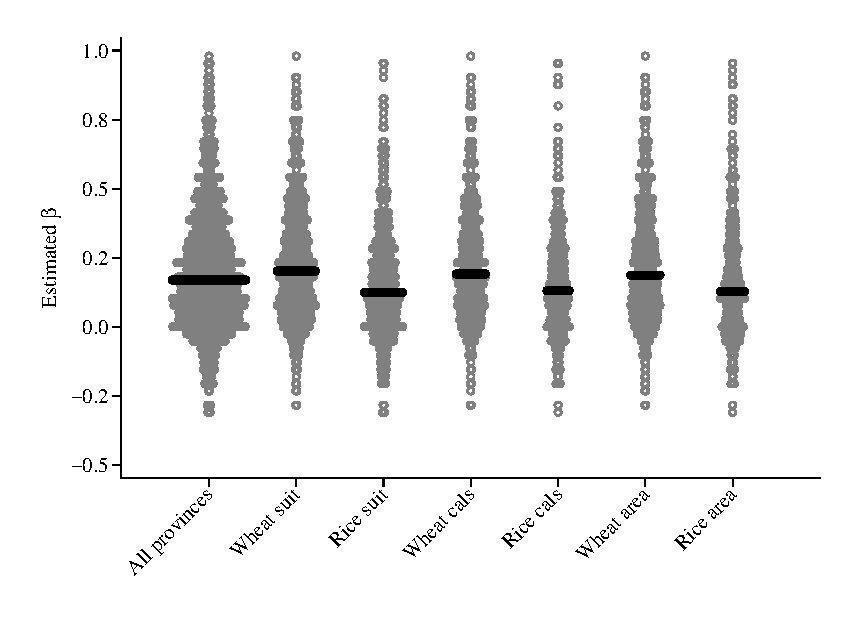
\includegraphics[width=.8\textwidth]{fig_beta_province.eps}
\end{center}
\end{frame}

\begin{frame}{Relationship of $\beta$ to rural density, by province}\label{rurdbeta}
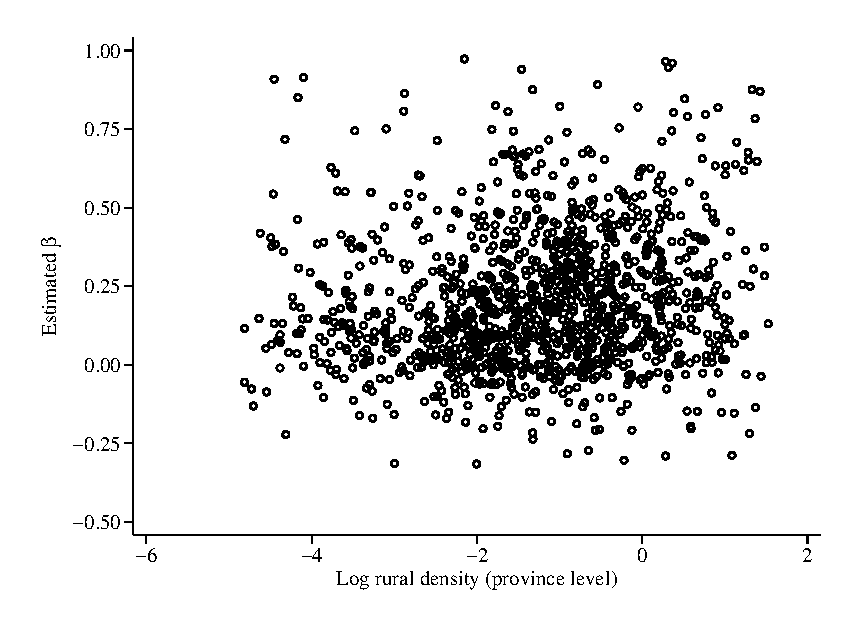
\includegraphics[width=.8\textwidth]{fig_beta_rurd.eps}
\hfill \hyperlink{eos}{\beamerbutton{Return}}
\end{frame}

\begin{frame}{Labor and capital not mobile}\label{nonmobile}
Factors cannot move within province, but output can.

\vspace{.2cm} Changes relationship of density and productivity to
\begin{equation}
  \ln A_{Ai} = \beta \ln L_{Ai}/X_i + \ln A_{Ni} + \alpha\beta \ln K_i/L_i + \ln p_N/p_A \nonumber
\end{equation}
\begin{itemize}
  \item Night lights provide proxy for $A_{Ni}$ and $K_i/L_i$?
  \item $p_N/p_A$ is province-specific (FE)
  \item Is correlation of $A_{Ni}$ and $K_i/L_i$ with $L_{Ai}/X_i$ different by climate zone?
\end{itemize}

\hfill \hyperlink{robustness}{\beamerbutton{Return}}
\end{frame}

\begin{frame}{Districts are autarkic}\label{autarky}
Factors and output are immobile within province.

\vspace{.2cm} Changes relationship of density and productivity to
\begin{equation}
\ln A_i = \beta \ln L_{Ai}/X_i - \ln L_{A_i}/L_i - \alpha(1-\beta) \ln K_{i}/L_{i} + \ln c_{Ai} \nonumber
\end{equation}
\begin{itemize}
  \item Can control for $L_{Ai}/L_i$ using HYDE data
  \item Night lights provide proxy for $K_i/L_i$?
  \item $c_{Ai}$ doesn't vary much and/or proxied by night lights?
\end{itemize}

\hfill \hyperlink{robustness}{\beamerbutton{Return}}
\end{frame}

\begin{frame}{Crop Results}

{\footnotesize
\begin{tabularx}{\textwidth}{lXXXXXX}
\midrule
\multicolumn{7}{l}{Dependent Variable in all panels: Log caloric yield ($A_{isc}$)} \\ \\
\multicolumn{7}{l}{Panel A: Samples defined by crop family (wheat vs. rice):} \\ \\
 & \multicolumn{2}{c}{By suitability:} & \multicolumn{2}{c}{By max calories:} & \multicolumn{2}{c}{By harvest area:}\\ \cmidrule(lr){2-3} \cmidrule(lr){4-5} \cmidrule(lr){6-7} 
 & Wheat & Rice & Wheat  & Rice  & Wheat  & Rice \\
 & Only & Only &  $>33\%$ & $>33\%$ & $>50\%$ & $>50\%$   \\
 & (1) & (2) & (3) & (4) & (5) & (6) \\
\midrule
Log rural density   &       0.254&       0.148&       0.213&       0.120&       0.231&       0.136\\
                    &     (0.024)&     (0.019)&     (0.021)&     (0.020)&     (0.020)&     (0.015)\\
\midrule
p-value $\beta=0$   &       0.000&       0.000&       0.000&       0.000&       0.000&       0.000\\
p-value $\beta=\beta^{Wheat}$&            &       0.001&            &       0.001&            &       0.000\\
Countries           &          91&          79&          82&          71&          74&          84\\
Observations        &        9922&        8396&       10142&        7411&        9929&        6810\\
Adjusted R-square   &        0.25&        0.21&        0.22&        0.18&        0.21&        0.18\\

\midrule
\end{tabularx}
}

\end{frame}

\begin{frame}{Using Cultivated Area}\label{cultreg}
Cultivated area, $X^C_{isc}$, available from GAEZ. Rural density is
\begin{equation}
  \ln L_{Aisc}/X_{isc} = \ln L_{Aisc}/X^C_{isc} + \ln X^C_{isc}/X_{isc}
\end{equation}

\begin{itemize}
  \item Regress $\ln A_{isc}$ on both terms on the right hand-side 
  \item Coefficient on $\ln L_{Aisc}/X^C_{isc}$ gives similar results for $\beta$
  \item Controls for percent of land actually being cultivated
\end{itemize}

\hfill \hyperlink{robustness}{\beamerbutton{Return}}
\end{frame}

%\begin{frame}{Measurement error?}
%\begin{itemize}
%  \item Whether we are using cultivated or total area
%  \item Systematic mismeasurement of districts within a province not a problem, FE
%  \item Variation in systematic mismeasurement across provinces not a problem, FE
%  \item Problem is \textit{variation in noise of mismeasurement} across provinces
%  \item Is there noisier measurement in tropical areas? 
%\end{itemize}
%\end{frame}

\begin{frame}{Using Cultivated Area}

{\footnotesize
\begin{tabularx}{\textwidth}{lXXXXXX}
\midrule
\multicolumn{7}{l}{Dependent Variable in all panels: Log caloric yield ($A_{isc}$)} \\ \\
\multicolumn{7}{l}{Panel A: Samples defined by crop family (wheat vs. rice):} \\ \\
 & \multicolumn{2}{c}{By suitability:} & \multicolumn{2}{c}{By max calories:} & \multicolumn{2}{c}{By harvest area:}\\ \cmidrule(lr){2-3} \cmidrule(lr){4-5} \cmidrule(lr){6-7} 
 & Wheat & Rice & Wheat  & Rice  & Wheat  & Rice \\
 & Only & Only &  $>33\%$ & $>33\%$ & $>50\%$ & $>50\%$   \\
 & (1) & (2) & (3) & (4) & (5) & (6) \\
\midrule
Log rural density   &       0.229&       0.144&       0.191&       0.113&       0.207&       0.142\\
                    &     (0.024)&     (0.020)&     (0.020)&     (0.021)&     (0.020)&     (0.015)\\
\midrule
p-value $\beta=0$   &       0.000&       0.000&       0.000&       0.000&       0.000&       0.000\\
p-value $\beta=\beta^{Wheat}$&            &       0.006&            &       0.006&            &       0.010\\
Countries           &          90&          76&          82&          68&          74&          81\\
Observations        &        9871&        8295&       10100&        7343&        9911&        6749\\
Adjusted R-square   &        0.20&        0.17&        0.17&        0.15&        0.16&        0.15\\

\midrule
\end{tabularx}
}

\end{frame}

\begin{frame}{Province-level Data}\label{regprov}

{\footnotesize
\begin{tabularx}{\textwidth}{lXXXXXX}
\midrule
\multicolumn{7}{l}{Dependent Variable in all panels: Log caloric yield ($A_{isc}$)} \\ \\
\multicolumn{7}{l}{Panel A: Samples defined by crop family (wheat vs. rice):} \\ \\
 & \multicolumn{2}{c}{By suitability:} & \multicolumn{2}{c}{By max calories:} & \multicolumn{2}{c}{By harvest area:}\\ \cmidrule(lr){2-3} \cmidrule(lr){4-5} \cmidrule(lr){6-7} 
 & Wheat & Rice & Wheat  & Rice  & Wheat  & Rice \\
 & Only & Only &  $>33\%$ & $>33\%$ & $>50\%$ & $>50\%$   \\
 & (1) & (2) & (3) & (4) & (5) & (6) \\
\midrule
Log rural density   &       0.399&       0.070&       0.248&       0.016&       0.368&       0.052\\
                    &     (0.058)&     (0.020)&     (0.030)&     (0.013)&     (0.043)&     (0.021)\\
\midrule
p-value $\beta=0$   &       0.000&       0.000&       0.000&       0.199&       0.000&       0.014\\
p-value $\beta=\beta^{Wheat}$&            &       0.000&            &       0.000&            &       0.000\\
Countries           &          60&          65&          70&          63&          69&          73\\
Observations        &         417&         587&         768&         617&         797&         721\\
Adjusted R-square   &        0.39&        0.27&        0.29&        0.26&        0.35&        0.30\\

\midrule
\end{tabularx}
}

\hfill \hyperlink{robustness}{\beamerbutton{Return}}
\end{frame}

\begin{frame}{Population Data from 1900}\label{reg1900}

{\footnotesize
\begin{tabularx}{\textwidth}{lXXXXXX}
\midrule
\multicolumn{7}{l}{Dependent Variable in all panels: Log caloric yield ($A_{isc}$)} \\ \\
\multicolumn{7}{l}{Panel A: Samples defined by crop family (wheat vs. rice):} \\ \\
 & \multicolumn{2}{c}{By suitability:} & \multicolumn{2}{c}{By max calories:} & \multicolumn{2}{c}{By harvest area:}\\ \cmidrule(lr){2-3} \cmidrule(lr){4-5} \cmidrule(lr){6-7} 
 & Wheat & Rice & Wheat  & Rice  & Wheat  & Rice \\
 & Only & Only &  $>33\%$ & $>33\%$ & $>50\%$ & $>50\%$   \\
 & (1) & (2) & (3) & (4) & (5) & (6) \\
\midrule
Log rural density   &       0.294&       0.170&       0.239&       0.149&       0.258&       0.182\\
                    &     (0.032)&     (0.025)&     (0.023)&     (0.025)&     (0.026)&     (0.017)\\
\midrule
p-value $\beta=0$   &       0.000&       0.000&       0.000&       0.000&       0.000&       0.000\\
p-value $\beta=\beta^{Wheat}$&            &       0.002&            &       0.007&            &       0.014\\
Countries           &          91&          81&          83&          71&          74&          84\\
Observations        &       10644&        9081&       10774&        8213&       10689&        7561\\
Adjusted R-square   &        0.30&        0.25&        0.25&        0.22&        0.24&        0.22\\

\midrule
\end{tabularx}
}

\hfill \hyperlink{robustness}{\beamerbutton{Return}}
\end{frame}

\begin{frame}{Above 25th Percentile Harvested Area}\label{harvarea}

{\footnotesize
\begin{tabularx}{\textwidth}{lXXXXXX}
\midrule
\multicolumn{7}{l}{Dependent Variable in all panels: Log caloric yield ($A_{isc}$)} \\ \\
\multicolumn{7}{l}{Panel A: Samples defined by crop family (wheat vs. rice):} \\ \\
 & \multicolumn{2}{c}{By suitability:} & \multicolumn{2}{c}{By max calories:} & \multicolumn{2}{c}{By harvest area:}\\ \cmidrule(lr){2-3} \cmidrule(lr){4-5} \cmidrule(lr){6-7} 
 & Wheat & Rice & Wheat  & Rice  & Wheat  & Rice \\
 & Only & Only &  $>33\%$ & $>33\%$ & $>50\%$ & $>50\%$   \\
 & (1) & (2) & (3) & (4) & (5) & (6) \\
\midrule
Log rural density   &       0.226&       0.140&       0.186&       0.111&       0.213&       0.125\\
                    &     (0.025)&     (0.020)&     (0.017)&     (0.021)&     (0.018)&     (0.013)\\
\midrule
p-value $\beta=0$   &       0.000&       0.000&       0.000&       0.000&       0.000&       0.000\\
p-value $\beta=\beta^{Wheat}$&            &       0.008&            &       0.005&            &       0.000\\
Countries           &          82&          65&          77&          58&          70&          72\\
Observations        &        7568&        6092&        7540&        5374&        8400&        5704\\
Adjusted R-square   &        0.22&        0.18&        0.19&        0.16&        0.19&        0.16\\

\midrule
\end{tabularx}
}

\hfill \hyperlink{robustness}{\beamerbutton{Return}}
\end{frame}

\begin{frame}{Maize and Soy Results}\label{othercrop}

{\footnotesize
\begin{tabularx}{\textwidth}{lXXXXXX}
\midrule
\multicolumn{7}{l}{Dependent Variable in all panels: Log caloric yield ($A_{isc}$)} \\ \\
\multicolumn{7}{l}{Samples defined by suitability for each crop:} \\ \\
 & \multicolumn{3}{c}{Maize suitable AND:} & \multicolumn{3}{c}{Soy suitable AND:} \\ \cmidrule(lr){2-4} \cmidrule(lr){5-7}
 & Wheat & Rice & Wheat  & Wheat  & Rice  & Wheat \\
 & or Rice & Only & Only & or Rice & Only & Only   \\
 & (1) & (2) & (3) & (4) & (5) & (6) \\
\midrule
Log rural density   &       0.135&       0.142&       0.209&       0.136&       0.144&       0.216\\
                    &     (0.015)&     (0.018)&     (0.035)&     (0.015)&     (0.018)&     (0.034)\\
\midrule
p-value $\beta=0$   &       0.000&       0.000&       0.000&       0.000&       0.000&       0.000\\
p-value $\beta=\beta^{All}$&            &       0.760&       0.011&            &       0.721&       0.004\\
Countries           &         116&          77&          78&         117&          78&          61\\
Observations        &       14499&        8365&        6781&       14486&        8220&        6311\\
Adjusted R-square   &        0.12&        0.12&        0.15&        0.12&        0.12&        0.15\\

\midrule
\end{tabularx}
}

\hfill \hyperlink{robustness}{\beamerbutton{Return}}
\end{frame}

\begin{frame}{Measurement Error}\label{measure}
Measurement error $\Rightarrow$ attentuation bias
\begin{itemize}
  \item Population data from HYDE may not be accurate for districts
  \item Is measurement error more pronounced in some places (e.g. tropical areas) and driving results?
  \item Is true variance of $\ln L_{Aisc}/X_{isc}$ one-third of measured variance?
  \item Is rural population mis-stated by factor of $>2$ or $<0.5$?
\end{itemize}

\hfill \hyperlink{robustness}{\beamerbutton{Return}}
\end{frame}

\begin{frame}{Elasticity of Substitution?}\label{eos}
What if land and labor do not have elasticity of subs. equal to one?
\begin{itemize}
  \item Elasticity of output w.r.t. land depends on rural density $L_A/X$
  \item With EOS more than one, higher density, lower elasticity
  \item Do results fit this?
  \begin{itemize}
    \item South/SE Asia, some SS Afr are high density, low $\beta$
    \item ..but C/S America, other SS Afr are low density, low $\beta$
    \item ..but N America lowest density, not highest $\beta$
  \end{itemize}
\end{itemize}
\hfill \hyperlink{rurdbeta}{\beamerbutton{Density?}}
\hfill \hyperlink{robustness}{\beamerbutton{Return}}
\end{frame}

\begin{frame}{Factor shares}\label{shares}
Our $\beta$ does not correlate well with factor share data
\begin{itemize}
  \item Fuglie (2010) reports share for ``land and structures''
  \begin{itemize}
    \item 0.22-0.25 share for Brazil, India, Indonesia $>$ our estimates
    \item 0.22 share for China, aggregate number?
    \item 0.17-0.26 for US, ex-Soviet $\approx$ our estimates
  \end{itemize}
  \item Hayami, Ruttan, Southworth (1979) for Asia
    \begin{itemize}
      \item 0.3-0.4 shares for Taiwan, Japan, Korea, Philippines $>$ our estimates
    \end{itemize}
  \item Clark (2002) for England, long run
    \begin{itemize}
      \item 0.3-0.35 shares $>$ our estimate for Northwest Europe
    \end{itemize}
\end{itemize}
\end{frame}

\begin{frame}{Factor Shares}
Possible sources of difference
\begin{itemize}
  \item Biased estimates of $\beta$
  \item Market frictions/wedges for agricultural inputs
  \item Mis-reporting of land versus labor income
  \item Difference of aggregate elasticity from farm-specific elasticity/share
\end{itemize}

\hfill \hyperlink{robustness}{\beamerbutton{Return}}
\end{frame}

\begin{frame}{Using IPUMS Population Data}\label{ipums}
39 countries in IPUMS with geographic identifiers for individuals at the ``district'' level (agglomerations of districts with constant boundaries). 
\begin{itemize}
  \item IPUMS gives industry/occupation and labor force status, so we can measure \textit{agricultural worker density}, not just rural density. In practice, rural density and ag worker density correlated at 91\%, sig at less than 1\%
  \item Counts of residents in each district are presumably more accurate that HYDE or GRUMP, as they are drawn from census. 
  \item Cost is limited coverage of countries, and fewer districts
  \item Rebuild data on $A_{isc}$ and $L_{Aisc}$ at the level of the IPUMS districts
\end{itemize}

\end{frame}

\begin{frame}{Using IPUMS Population Data}

{\footnotesize
\begin{tabularx}{\textwidth}{lXXXXXX}
\midrule
\multicolumn{7}{l}{Dependent Variable in all panels: Log caloric yield ($A_{isc}$)} \\ \\
\multicolumn{7}{l}{Panel A: Samples defined by crop family (wheat vs. rice):} \\ \\
 & \multicolumn{2}{c}{By suitability:} & \multicolumn{2}{c}{By max calories:} & \multicolumn{2}{c}{By harvest area:}\\ \cmidrule(lr){2-3} \cmidrule(lr){4-5} \cmidrule(lr){6-7} 
 & Wheat & Rice & Wheat/  & Rice  & Wheat  & Rice \\
 & Only & Only &  No Rice & No Wheat & $>50\%$ & $>50\%$   \\
 & (1) & (2) & (3) & (4) & (5) & (6) \\
\midrule
Log ag. worker density&       0.213&       0.025&       0.200&       0.000&       0.223&       0.034\\
                    &     (0.067)&     (0.016)&     (0.056)&     (0.017)&     (0.030)&     (0.014)\\
\midrule
p-value $\beta=0$   &       0.004&       0.124&       0.002&       0.993&       0.000&       0.021\\
p-value $\beta=\beta^{Wheat}$&            &       0.006&            &       0.000&            &       0.000\\
Countries           &          23&          24&          24&          23&          21&          26\\
Observations        &        1104&        2416&        1595&        2389&        1207&        1427\\
Adjusted R-square   &        0.50&        0.54&        0.39&        0.56&        0.37&        0.51\\

\midrule
\end{tabularx}
}

\hfill \hyperlink{robustness}{\beamerbutton{Return}}
\end{frame}

\begin{frame}{Using GRUMP Population Data}\label{grump}
GRUMP (Global Rural-Urban Mapping Project) also provides grid-cell population estimates. 
\begin{itemize}
  \item Define urban/rural differently than HYDE. They denote specific grid-cells as ``urban'', and any population in that cell is assumed to be urban.
  \item Inclusion of cells in districts and provinces is identical to HYDE. 
\end{itemize}
\end{frame}

\begin{frame}{Using GRUMP Population Data}

{\footnotesize
\begin{tabularx}{\textwidth}{lXXXXXX}
\midrule
\multicolumn{7}{l}{Dependent Variable in all panels: Log caloric yield ($A_{isc}$)} \\ \\
\multicolumn{7}{l}{Panel A: Samples defined by crop family (wheat vs. rice):} \\ \\
 & \multicolumn{2}{c}{By suitability:} & \multicolumn{2}{c}{By max calories:} & \multicolumn{2}{c}{By harvest area:}\\ \cmidrule(lr){2-3} \cmidrule(lr){4-5} \cmidrule(lr){6-7} 
 & Wheat & Rice & Wheat/  & Rice  & Wheat  & Rice \\
 & Only & Only &  No Rice & No Wheat & $>50\%$ & $>50\%$   \\
 & (1) & (2) & (3) & (4) & (5) & (6) \\
\midrule
Log rural density   &       0.207&       0.115&       0.176&       0.100&       0.166&       0.140\\
                    &     (0.041)&     (0.021)&     (0.033)&     (0.017)&     (0.028)&     (0.020)\\
\midrule
p-value $\beta=0$   &       0.000&       0.000&       0.000&       0.000&       0.000&       0.000\\
p-value $\beta=\beta^{Wheat}$&            &       0.045&            &       0.041&            &       0.442\\
Countries           &          86&          75&          81&          69&          71&          82\\
Observations        &        8734&        6769&        8585&        6230&        8922&        5844\\
Adjusted R-square   &        0.19&        0.16&        0.15&        0.13&        0.14&        0.13\\

\midrule
\end{tabularx}
}

\hfill \hyperlink{robustness}{\beamerbutton{Return}}
\end{frame}

\end{document}
